\subsection*{2 a)}
\textbf{Finn strømlinjene.}
\\
\\
Vi har fått oppgitt hastighetsfeltet:

\begin{align*}
    \textbf{v} = v_x\textbf{i} + v_y \textbf{j} =  xy\textbf{i} + y \textbf{j}
\end{align*}

Det er også gitt hint om at denne kan være separabel og vi vet fra
GF at $v_x \dd x = v_y \dd y$ er en nyttig relasjon for å finne strømlinjene:

\begin{align*}
    v_x \dd y &= v_y \dd x
    \\
    xy \dd y &= y\dd x
    \\
    x\dd y &= 1\dd x
    \\
    \int 1 \dd y &= \int \frac{1}{x} \dd x
    \\
    y &= \log(x) + C_0
    \\
    y - \log(x) &= C
\end{align*}















\pagebreak
\subsection*{2 b)}

\textbf{Tegn strømlinjene \sout{for hånd} og sett på piler
for å indikere retningen på strømmen. Et stagnasjonspunkt er et
punkt hvor hastighetsfeltet er lik null. Finn alle stagnasjonspunktene
og identifiser hvor i plottet disse ligger. Det er vanlig å tegne
individuelle stagnasjonspunkter som tjukke kulepunkter.
\\
\\
Vis også at du får til å tegne strømlinjene ved hjelp av
\sout{Matlab eller} Python. Dette kan kanskje vise seg å være en utfordring nær x = 0.}

\begin{figure}[H]
		\centering
		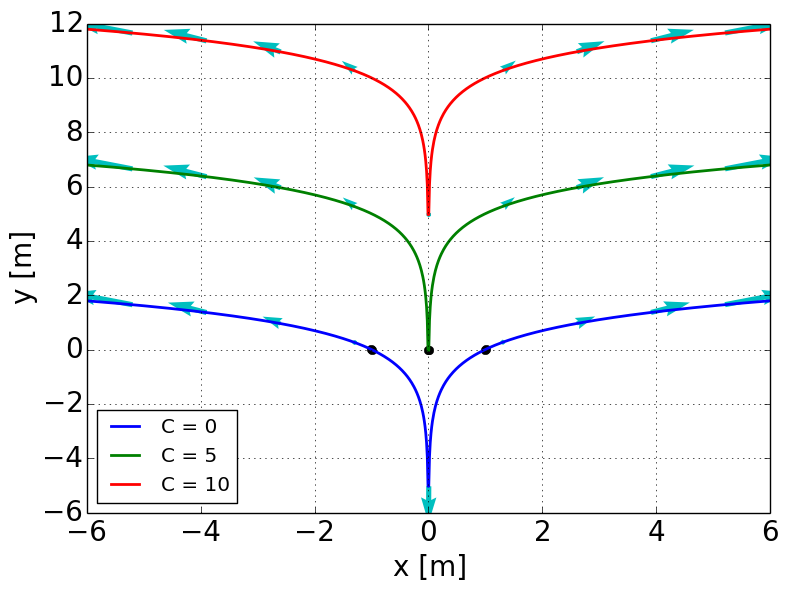
\includegraphics[width=0.7\linewidth]{../2b.png}
		\caption{Figuren viser tre kurver med forskjellige $C$.
        På kurvene er strømvektorene vist som lyseblå vektorer
         og stagnasjonspunkter er vist som svarte prikker.}
		\label{fig_2b_test}
\end{figure}

Figur \ref{fig_2b_test} viser strømlinjene til hastighetsfeltet som
ble oppgitt i oppgave 2. Langs strømlinjene er strømvektorene også
tegnet. Retningen til strømvektorene er tangentiell til strømlinjene.
Det er uendelig mange stagnasjonspunkter langs x-aksen, hvor to og to hører
til en C-verdi.
\\
\\
Jeg glemte å tegne for hånd.








\pagebreak
\subsection*{2 c)}
\textbf{Vis at det ikke finnes en strømfunksjon $\psi$.}
\\
\\
Det blir gitt hint om at det er to måter å vise at feltet ikke har en
strøm funksjon. Regn ut strømfunksjonen og vis at det er en selvmotsigelse
eller hvis at divergensen er ulik null.
\\
\\
Vi skal selvfølgelig gjøre begge:
\\
\\
\\
\begin{align*}
    &v_x = -\partial \psi / \partial y
    && v_y = \partial \psi / \partial x
    \\
    &\psi = -\int v_x \dd y
    &&\psi = \int v_y \dd x
    \\
    &\psi = -\int xy \dd y
    &&\psi = \int y \dd x
    \\
    &\psi = - \frac{1}{2} xy^2
    &&\psi =  xy
\end{align*}

Dette er en åpenbar selvmotsigelse. $\psi$ kan ikke være så bipolar at den
er $xy$ og $- \frac{1}{2} xy^2$ samtidig.
\\
\\
\\
\\

Divergensen er lik $\nabla \cdot \textbf{v} = \partial v_x /\partial x
+  \partial v_y /\partial y$. Med hastighetsfeltet vårt gir det:

\begin{align*}
    \frac{\partial v_x}{\partial x}
    +
    \frac{\partial v_y}{\partial y}
    &=
    \frac{\partial xy}{\partial x}
    +
    \frac{\partial y}{\partial y}
    \\
    \\
    \frac{\partial xy}{\partial x}
    =
    y
    &\qquad \qquad
    \frac{\partial y}{\partial y}
    =
    1
    \\
    \\
    \nabla \cdot \textbf{v} &= \underline{\underline{y + 1 \neq 0}}
    \\
    \\
\end{align*}






%
